\documentclass[letterpaper,9pt,twoside,printwatermark=false]{pinp}

%% Some pieces required from the pandoc template
\providecommand{\tightlist}{%
  \setlength{\itemsep}{0pt}\setlength{\parskip}{0pt}}

% Use the lineno option to display guide line numbers if required.
% Note that the use of elements such as single-column equations
% may affect the guide line number alignment.

\usepackage[T1]{fontenc}
\usepackage[utf8]{inputenc}

% The geometry package layout settings need to be set here...
\geometry{layoutsize={0.95588\paperwidth,0.98864\paperheight},%
          layouthoffset=0.02206\paperwidth,%
		  layoutvoffset=0.00568\paperheight}

\definecolor{pinpblue}{HTML}{185FAF}  % imagecolorpicker on blue for new R logo
\definecolor{pnasbluetext}{RGB}{101,0,0} %



\title{Assignment 6 - Power, Sample Size and Inference for a Population
Proportion. Due October 26, 5:00pm 2018}

\author[a]{EPIB607 - Inferential Statistics}

  \affil[a]{Fall 2018, McGill University}

\setcounter{secnumdepth}{5}

% Please give the surname of the lead author for the running footer
\leadauthor{Bhatnagar and Hanley}

% Keywords are not mandatory, but authors are strongly encouraged to provide them. If provided, please include two to five keywords, separated by the pipe symbol, e.g:
 \keywords{  Power |  Sample Size |  Binomial Distribution |  One sample proportion |  Bootstrap  }  

\begin{abstract}
In this assignment you will practice conducting inference for a one
sample proportion as well as conducting power and sample size
calculations. Answers should be given in full sentences (DO NOT just
provide the number). All figures should have appropriately labeled axes,
titles and captions (if necessary). Units for means and CIs should be
provided. State your hypotheses and assumptions when applicable. All
graphs and calculations are to be completed in an R Markdown document
using the provided template. You are free to choose any function from
any package to complete the assignment. Concise answers will be
rewarded. Be brief and to the point. Please submit both the compiled
HTML report and the source file (.Rmd) to myCourses by October 26, 2018,
5:00pm. Both HTML and .Rmd files should be saved as
`IDnumber\_LastName\_FirstName\_EPIB607\_A6'.
\end{abstract}

\dates{This version was compiled on \today}
\doi{\url{https://sahirbhatnagar.com/EPIB607/}}

\pinpfootercontents{Assignment 6 due October 26, 2018 by 5:00pm}

\begin{document}

% Optional adjustment to line up main text (after abstract) of first page with line numbers, when using both lineno and twocolumn options.
% You should only change this length when you've finalised the article contents.
\verticaladjustment{-2pt}

\maketitle
\thispagestyle{firststyle}
\ifthenelse{\boolean{shortarticle}}{\ifthenelse{\boolean{singlecolumn}}{\abscontentformatted}{\abscontent}}{}

% If your first paragraph (i.e. with the \dropcap) contains a list environment (quote, quotation, theorem, definition, enumerate, itemize...), the line after the list may have some extra indentation. If this is the case, add \parshape=0 to the end of the list environment.


\section*{Template}\label{template}
\addcontentsline{toc}{section}{Template}

The \texttt{.Rmd} template for Assignment 6 is available
\href{https://github.com/sahirbhatnagar/EPIB607/raw/master/assignments/a6/a6_template.Rmd}{here}

\section{Bias in step counters}\label{bias-in-step-counters}

Following the study by
\href{http://www.medicine.mcgill.ca/epidemiology/hanley/bios601/Surveys/SmartphoneSteps.pdf}{Case
et al., JAMA, 2015}, suppose we wished to assess, via a formal
statistical test, whether (at an \textit{population}, rather than an
individual, level) a step-counting device or app is unbiased (\(H_0\))
or under-counts (\(H_1\)). Suppose we will do so the way
\href{http://www.medicine.mcgill.ca/epidemiology/hanley/bios601/Surveys/SmartphoneSteps.pdf}{Case
et al.} did, but measuring \(n\) persons just once each. We observe the
device count when the true count on the treadmill reaches 500.

\begin{enumerate}
\def\labelenumi{\alph{enumi}.}
\tightlist
\item
  Using a planned sample size of \(n=25\), and \(\sigma = 60\) steps as
  a pre-study best-guess as to the \(s\) that might be observed in them,
  calculate the critical value at \(\alpha = 0.01\).
\item
  Now imagine that the mean would not be the null 500, but \(\mu=470.\)
  Calculate the probability that the mean in the sample of 25 will be
  less than this critical value. Use the same \(s\) for the alternative
  that you used for the null. What is this probability called?
\item
  Determine the sample size required for 80\% power using a 1\% level of
  significance. Plot the null and alternative distributions in a diagram
  using the
  \href{https://raw.githubusercontent.com/sahirbhatnagar/EPIB607/master/assignments/a6/plot_null_alt.R}{\texttt{plot\_power}}
  function. An example of how to use this function and its output is
  shown below:
\end{enumerate}

\begin{Shaded}
\begin{Highlighting}[]
\KeywordTok{source}\NormalTok{(}\StringTok{"https://raw.githubusercontent.com/sahirbhatnagar/EPIB607/master/assignments/a6/plot_null_alt.R"}\NormalTok{)}

\NormalTok{mu0 <-}\StringTok{ }\FloatTok{-0.540} \CommentTok{# mean under the null}
\NormalTok{mha <-}\StringTok{ }\FloatTok{0.99}\OperatorTok{*-}\FloatTok{0.540} \CommentTok{# mean under the alternative}
\NormalTok{s <-}\StringTok{ }\FloatTok{0.0080} \CommentTok{# sample/population SD}
\NormalTok{n <-}\StringTok{ }\DecValTok{5} \CommentTok{# sample size}
\NormalTok{cutoff <-}\StringTok{ }\NormalTok{mu0 }\OperatorTok{+}\StringTok{ }\KeywordTok{qnorm}\NormalTok{(}\FloatTok{0.95}\NormalTok{) }\OperatorTok{*}\StringTok{ }\NormalTok{s }\OperatorTok{/}\StringTok{ }\KeywordTok{sqrt}\NormalTok{(n)}

\KeywordTok{power_plot}\NormalTok{(}\DataTypeTok{n =}\NormalTok{ n, }
           \DataTypeTok{s =}\NormalTok{ s,  }
           \DataTypeTok{mu0 =}\NormalTok{ mu0, }
           \DataTypeTok{mha =}\NormalTok{ mha, }
           \DataTypeTok{cutoff =}\NormalTok{ cutoff,}
           \DataTypeTok{alternative =} \StringTok{"greater"}\NormalTok{,}
           \DataTypeTok{xlab =} \StringTok{"Freezing point (degrees C)"}\NormalTok{)}
\end{Highlighting}
\end{Shaded}

\begin{ShadedResult}
\begin{verbatim}
#  Loading required namespace: latex2exp
\end{verbatim}
\end{ShadedResult}

\begin{center}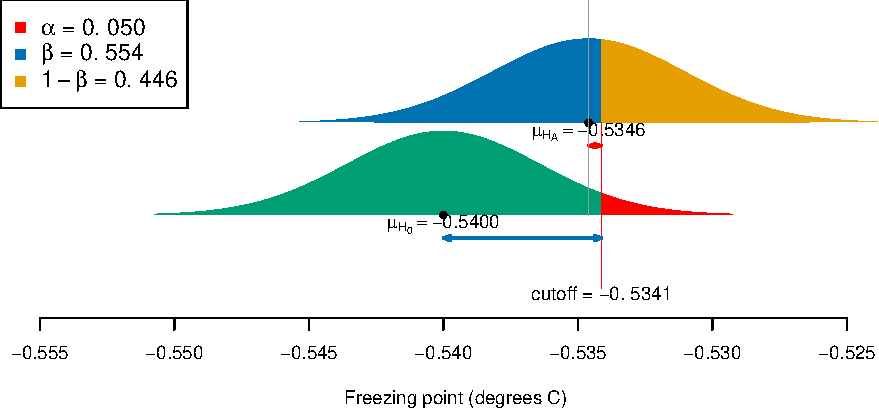
\includegraphics{a6_power_proportions_files/figure-latex/unnamed-chunk-1-1} \end{center}

\section{Boosting sales}\label{boosting-sales}

You want to see if a redesign of the cover of a mail-order catalog will
increase sales. A very large number of customers will receive the
original catalog and a random sample of customers will receive the one
with the new cover. For planning purposes, you are willing to assume
that the sales from the new catalog will be approximately normal with
\(\sigma=50\) dollars and that the mean for the original catalog will be
\(\mu = 25\) dollars. You decide to use a sample size of \(n = 900\).
You wish to test \[H_0: \mu = 25 \qquad H_a: \mu > 25\]You decide to
reject \(H_0\) if \(\bar{y} > 26\) and fail to reject \(H_0\) otherwise.

\begin{enumerate}
\def\labelenumi{\alph{enumi}.}
\tightlist
\item
  Find the probability of a Type I error.
\item
  Find the probability of a Type II error when \(\mu = 28\) dollars.
\item
  Find the probability of a Type II error when \(\mu = 30\) dollars.
\item
  The distribution of sales is not normal because many customers buy
  nothing. Why is it nonetheless reasonable in this circumstance to
  assume that the mean will be approximately normal?
\end{enumerate}

\section{Fill the bottles}\label{fill-the-bottles}

Bottles of a popular cola drink are supposed to contain 300 milliliters
(ml) of cola. There is some variation from bottle to bottle because the
filling machinery is not perfectly precise. Assume the standard
deviation (\(\sigma\)) of the filling process is 3 ml. An inspector, who
suspects that the bottler is underfilling, measures the contents of a
sample of six bottles. Power calculations help us see how large a
shortfall in the bottle contents the test can be expected to detect.

\begin{enumerate}
\def\labelenumi{\alph{enumi}.}
\tightlist
\item
  Find the power of a 5\% significance test against the alternative
  \(\mu= 299\) ml.
\item
  Find the power against the alternative \(\mu = 295\) ml.
\item
  Is the power against \(\mu = 290\) higher or lower than the value you
  found in (b)? Explain why this result makes sense.
\item
  Make a plot of the power as a function of the shortfall (\(\Delta\)),
  and comment on the plot.
\end{enumerate}

\section{Drunken cyclists}\label{drunken-cyclists}

In the United States approximately 900 people die in bicycle accidents
each year. One study examined the records of 1711 bicyclists aged 15 or
older who were fatally injured in bicycle accidents between 1987 and
1991 and were tested for alcohol. Of these, 542 tested positive for
alcohol (blood alcohol concentration of 0.01\% or higher).

\begin{enumerate}
\def\labelenumi{\alph{enumi}.}
\tightlist
\item
  To do statistical inference for these data, we think in terms of a
  model where \(p\) is parameter that represents the probability that a
  tested bicycle rider is positive for alcohol. Find a 99\% confidence
  interval for \(p\).
\item
  Can you conclude from your analysis of this study that alcohol causes
  fatal bicycle accidents? Explain
\item
  In this study 386 bicyclists had blood alcohol levels above 0.10\%, a
  level defining legally drunk in many states at the time. Give a 99\%
  confidence interval for the proportion who were legally drunk
  according to this criterion.
\end{enumerate}

\newpage

\section{Handling contact lenses}\label{handling-contact-lenses}

Failure to follow recommended contact lens wear and care practices can
lead to serious eye infection. A survey of a random sample of 281
Americans who wear contact lenses regularly asked about contact lens
practices. The survey found that 139 respondents do not consistently
wash their hands before handing their contact lenses.

\begin{enumerate}
\def\labelenumi{\alph{enumi}.}
\tightlist
\item
  Obtain a plus four 99\% confidence interval for the proportion \(p\)
  of all American contact lens wearers who do not consistently wash
  their hands before handing their lenses. Verify that the conditions
  for your confidence interval are met.
\item
  Obtain a large sample 99\% confidence interval for the proportion
  \(p\) of all American contact lens wearers who do not consistently
  wash their hands before handing their lenses. How does this compare to
  the interval you calculated in part (a)?
\item
  The researchers indicated that this survey had a substantial
  nonresponse rate. How does this information affect your interpretation
  of the confidence interval in context?
\item
  Survey participants simply answered a questionnaire, and no attempt
  was made to verify the answers. How does this information affect your
  interpretation of the confidence interval in context?
\end{enumerate}

\section{Cancer-detecting dogs}\label{cancer-detecting-dogs}

A study was designed to determine whether dogs can be trained to
identify urine specimens from individuals with bladder cancer. Dogs were
first trained to discriminate between urine specimens from patients with
bladder cancer and urine specimens from patients with other conditions.
After the training was completed, the dogs had to pick one of seven new
urine specimens. Each time, only one of the seven urine specimens came
from a patient with bladder cancer. Out of 54 trials, the dogs
identified the correct urine specimen 22 times.

\begin{enumerate}
\def\labelenumi{\alph{enumi}.}
\tightlist
\item
  If the dogs were simply picking a urine specimen at random, we would
  expect them to be correct, on average, 1 out of 7 times. The
  experiment was designed to test whether dogs can perform better than
  chance. State the null and alternative hypotheses for this test.
\item
  Obtain the test statistic and the P-value. What do you conclude?
\end{enumerate}

%\showmatmethods


\bibliography{pinp}
\bibliographystyle{jss}



\end{document}

